% don't remove the folling lines, and edit the defintion of \main if needed
\documentclass[../report.tex]{subfiles}
\providecommand{\main}{..}
\IfEq{\jobname}{\currfilebase}{\AtEndDocument{\biblio}}{}
% until here


\begin{document}
\linenumbers
% this is the extra information to be used for the general sections.
\chapter{Flavour Physics}
\label{chap:flav}

This chapter discusses the present and future flavour quest, focusing first on the physics of the spectrum lighter than $\sim$\,GeV, and then on the heavier fermions, 
 the heavy SM bosons, and finally the flavour-dark sector connection. The terminology short-term, mid-term and long-term will denote, respectively, present experiments, updates of the latter (e.g.\ LHCb Upgrade~II) as well as approved projects (e.g.\ Belle II, HL-LHC, Mu3e, etc.), and future facilities under discussion.  

\section{Introduction/Theory of Flavour}
That fundamental forces arise as gauge interactions is experimentally an extremely successful prediction of the
Standard Model (SM) of particle physics. 
In contrast, within the SM 
a deep understanding of the rationale for the Higgs couplings and the flavour structure remains to be achieved.  There is a striking difference between the simplicity of the gauge sector, described by just three gauge couplings, and the complicated structure of the rest of the SM with over twenty Higgs related parameters describing the SM flavour structure. This  suggests that flavour physics
is  a unique portal to 
a more fundamental organizing principle. 


Further fundamental questions emerge when attempts are made to 
couple the SM and gravity. The quantization of the latter remains a crucial open question. In addition, the data 
 point towards a universe that cannot be understood solely in terms of the SM and gravity. 
There is strong evidence  for the existence of new particles and {\it new \underline{particle} physics} (NP): 
\begin{itemize}
    \item {\it Experimental evidence} which remains unexplained within the SM laws, to wit 
    \begin{enumerate}
        \item {\it Dark matter}, whose nature is unknown, and the mass range of possible dark matter candidates spanning across over eighty orders of magnitude. 
        \item {\it Neutrino masses}. The SM gauge group allows for Majorana neutrino masses, justifying their suppressed values, but the size of the putative Majorana
 scale is unknown.
        \item The observed {\it matter-antimatter asymmetry} of the Universe. 
    \end{enumerate}
    
   \vspace{0.2cm}
    
    \item {\it Strong tensions and fine-tunings within the SM}, such as   
    \begin{enumerate}
        \item {\it The electroweak (EW) hierarchy problem}. ``Why is the Higgs so light?''  when its mass is {\it a priori} sensitive through quantum corrections to any putative high scale.  What stabilizes  the Higgs vacuum expectation value? 
        \item {\it The strong CP problem}, that defines the QCD vaccuum.  Why is its $\theta$ parameter experimentally constrained to be extremely small? For {\it a priori} no good reason.
        \item {\it The flavour puzzle}. Why are there three generations of quarks and leptons? What accounts for the very different masses and mixings? What fixes the  
        size of CP-violation, largely insufficient to explain the observed dominance of matter over anti-matter?
    \end{enumerate}
     The flavour puzzle, in particular, feeds into the first two tensions. For instance, within the SM the top loop gives the main contribution to the EW hierarchy problem, while the strong CP problem is an issue only in as much as all the quarks have non-zero masses. Furthermore, many NP models designed to solve the EW hierarchy problem tend to worsen the strong CP problem and generate unacceptably large contributions to electric dipole moments (EDMs), 
    as a consequence
    of the presence of CP-violation in  non-chiral flavour changing couplings.  
      All three tensions in their core amount 
 to the question of why certain parameters are very small. 
 In natural theories small numbers are explained by  symmetries or dynamical assumptions, suggesting that the SM needs to be extended in order to become a natural theory. 
      \end{itemize} 
    
     The underlying nature of CP violation, which is at the heart of many open questions,
     deserves  
     special mention. On the one hand, the  combination of the discrete symmetries C, P and T is essential to the formulation of quantum field theory itself. On the other hand, CP violation  is at the backbone of the SM three-family flavour puzzle and of the strong CP problem. In addition,  it 
     is also an essential ingredient to generate the observed baryon asymmetry (assuming baryogenesis). From a 
     practical perspective, it is one of the main driving forces behind the present experimental efforts, especially in the neutrino sector. Finally,  dark matter itself may have flavour structure,   and 
     a true understanding of flavour would then require an interdisciplinary exploration. As a side benefit,  
      the present and planned flavour experiments  are  often, without special requirements, 
      sensitive to light dark matter candidates such as feebly interacting particles.
 
\begin{figure}
\begin{center}
\includegraphics[width=0.90\textwidth, angle=0]{\main/Flavour/figs/Sensitivity_plot_J_style}
\end{center}
\caption{Reach in new physics scale of present and future facilities, from generic dimension six operators. Colour coding of observables is: green for mesons, blue for leptons, yellow for EDMs, red for Higgs flavoured couplings and purple for the top quark. The grey columns illustrate the reach of direct flavour-blind searches and EW precision measurements.
The operator coefficients are taken to be either $\sim 1$ (plain coloured columns)
or suppressed by MFV factors (hatch filled surfaces). Light (dark) colours correspond to present data (mid-term prospects).
}\label{fig:NPscales}
\end{figure}
  
The progress in understanding the above fundamental questions can be made through a variety of tools: directly by  increasing the energy at which  the world of fundamental particles and forces is explored, or indirectly by making precise measurements of rare or even SM forbidden processes, relying on quantum mechanical effects to probe shorter distances or effectively higher energies.  
The expected experimental progress, especially with regards to the indirect probes,  can be  neatly encoded in the model-independent tool of effective Lagrangians. As long as the NP particles are heavier than the energy released in a given experiment, their impact can be included via effective operators of increasing mass dimensions, constructed from the SM fields. The resulting effective field theory (SM-EFT) has the following form: 
\begin{equation}
    \mathcal{L}_{\text{eff}}= \mathcal{L}_{\text{SM}} + \frac{C_5}{\Lambda_M}\mathcal{O}^{(5)} +  \sum_a \frac{C_{6}^{a}}{\Lambda^2}\mathcal{O}^{(6)}_{a}+\cdots \,. 
    \label{effective}
\end{equation}
The dimension five ($d=5$) operator $\mathcal{O}^{(5)}$  
breaks lepton number and, if present, induces Majorana neutrino masses of order  $v^2/\Lambda_M$, where  $\Lambda_M$ is assumed to be 
much larger than the electroweak (EW) scale $v$. The $d=6$ operators ${O}^{(6)}_{a}$  
encode the effects of  
NP particles of generic mass $\Lambda$. 
Experiments probe the ratios $C^a / \Lambda^2$. 

For a qualitative appraisal, Fig.~\ref{fig:NPscales} illustrates the scales probed  by the present flavour  experiments (light colours), assuming  $C_6^a\sim {\mathcal O}(1)$~\cite{Nir_Private}. This can be compared with the reach of direct high-energy searches and EW precision tests (in grey), illustrated  by using flavour-blind operators that have the optimal reach~\cite{Nir_Private}: the gluon-Higgs operator and the oblique parameters for EW precision tests, respectively.  The shown effective energy reach of flavour experiments do have several caveats. First of all, in many realistic theories either the coupling constants are  smaller than unity and/or the symmetries suppress the sizes of the coefficients.  This effect is illustrated by including in the quark sector the present bounds in tree level NP with Minimal Flavour Violation (MFV) pattern of couplings (hatch filled areas)~\cite{Chivukula:1987py,Buras:2000dm,DAmbrosio:2002vsn,Cirigliano:2005ck}. Furthermore, there could be cancellations among several higher-dimension operators. In addition, for theories in which the new physics contributes as an insertion inside a one-loop diagram mediated by SM particles,  
all the shown scales should be further reduced by extra
GIM-mass suppressions and/or
a factor $\alpha /4\pi \sim10^{-3}$ 
(where $\alpha$ denotes the generic gauge structure constants).

Finally and importantly, the  new physics scale behind the flavour paradigm may differ from the  electroweak new physics scale.  Despite these caveats, Fig.~\ref{fig:NPscales} does illustrate the unique power of flavour physics to probe NP.
 The next generation of precision particle physics experiments will probe significantly higher effective NP scales, as discussed in more detail below. 









  







    


 
 

\section {Light sector: spectrum below GeV (short-, mid- and long-term)}
\subsection{Electric dipole moments ($n$, $p$, charged leptons, atoms)}

Electric dipole moments  are the P- and CP-odd  
counterparts (from CPT conservation) to magnetic moments. They arise from a set of  ${O}^{(6)}_{a}$ operators in Eq.~(\ref{effective}) which flip the chirality of a fermion  and involve the EW field strengths and the Higgs doublet. After spontaneous symmetry breaking they result in a coupling 
of the fermion spin $\vec{\sigma}$ to the electric field $\vec{E}$ of the form $d\,\vec{\sigma} \cdot \vec{E}$, where $d$  denotes the  EDM strength.

\begin{figure}
\begin{center}
\includegraphics[width=0.43\textwidth]{\main/Flavour/figs/EDM_SM} \hspace*{5mm}
\raisebox{10mm}{\includegraphics[width=0.37\textwidth]{\main/Flavour/figs/EDM_SUSY} }
\end{center}
\caption{On the left, one example of SM contribution to the quark EDM; on the right, one-loop new physics contribution, exemplified by a generic supersymmetric  contribution mediated by squarks and gauginos. }\label{fig:FeynEDM} 
\end{figure}

The EDMs are clean and powerful probes of new physics (NP).  
In the SM, the
EW contributions to quark EDMs arise only at 3 loop-level and are
extremely suppressed due to the chiral nature of the SM flavour changing currents: the predictions lie well below present sensitivities. The same applies to leptons taking into account the known structure of neutrino masses and mixings. 
In contrast, most new physics models   
include new mediators and  new sources of CP violation that can generate  EDMs already at one-loop level, see Fig.~\ref{fig:FeynEDM}. The bounds on the EDMs thus severely constrain NP scenarios. For instance, 
in the absence of a suppression mechanism the new contributions to the EDMs can be easily in 
the range of $10^{-23}- 10^{-25}$~e$\cdot$cm, which is already in conflict with the present experimental bounds. Note that the EDMs are null searches; any nonzero signal at present or projected sensitivities would imply new physics.


The quark (or hadron) EDM and lepton EDM searches are complementary, as they may test different physics.  The leptonic  EDM is necessarily sourced by EW physics, while the hadronic EDMs are sensitive to both the EW and the strong interactions, for instance the $\theta$  parameter of QCD. 
The EDM searches are also
complementary to the high-energy CP probes, since they probe a different combination of NP parameters. 
 The combination of
quark and lepton searches for CP violation at different frontiers is
thus a formidable tool to test for NP. 





The current experimental limit on the {\bf neutron EDM} is
$d_n < 3.6 \times 10^{-26}$~e$\cdot$cm at $95\%$ CL~\cite{Chupp:2017rkp},
and for the {\bf electron EDM} $d_e < 1.1 \times 10^{-29}$~e$\cdot$cm at $90\%$
CL~\cite{Andreev:2018ayy}.  
These bounds already test NP at mass scales above $10$ TeV and up to $\sim 10^6$ TeV, see  Fig.~\ref{fig:NPscales} (light yellow columns).  
A variety of other systems 
have also been explored as sensitive probes 
of the EDMs: atoms, protons,  deuterons, muons and different molecules. The current status of the measurements is reported in   Table~\ref{tab:EDM_all}.
The European collaborations lead current neutron EDM searches~\cite{Afach:2015sja}, while the best limits using molecules~\cite{Andreev:2018ayy}, 
diamagnetic atoms~\cite{Graner:2016ses} and 
muons~\cite{Bennett:2008dy} presently come from the experiments conducted in the USA. 

{\setlength{\tabcolsep}{2pt} % Default value: 6pt
\begin{table}
\caption{Current EDM limits. In the table, $Q_m$ denotes the magnetic quadrupole moment, $C_S$ is the scalar form factor, and  $\mu_N$ and $R_{Cs}$ are the nuclear magneton and the nuclear radius of $^{133}C_s$, respectively. For 
further details and a complete review of the experimental 
scenarios see Ref.~\cite{Chupp:2017rkp}. } 
\label{tab:EDM_all} 
{\scriptsize
 \begin{center}
\begin{tabular}{cc}
 \begin{tabular}{lll}
\hline\hline
 & Result & 95\% u.l.\\ \hline 
 \\
& $\quad$ Paramagnetic  systems
 & \\ 
 \hline
 \\
Xe$^m$ & $d_A = (0.7\pm 1.4)\times 10^{-22}$ & $3.1 \times 10^{-22}$ 
e\, cm\\
Cs & $d_A =(-1.8 \pm 6.9) \times 10^{-24}$ &
$1.4 \times 10^{-23}$ 
e\, cm\\ 
& $d_e =(-1.5 \pm 5.7) \times 10^{-26}$& $1.2 \times 10^{-25}$ e\, cm\\ 
& $C_S =(2.5 \pm 9.8) \times 10^{-6}$& $2 \times 10^{-5}$\\
& $Q_m =(3 \pm 13) \times 10^{-8}$& $2.6 \times 10^{-7}$ $\mu_N R_{\rm{Cs}}$\\
Tl &$d_A =(-4.0\pm 4.3) \times 10^{-25}$ & $1.1 \times 10^{-24}$ e\, cm \\
& $d_e =(6.9 \pm 7.4) \times 10^{-28}$& $1.9 \times 10^{-27}$ e\, cm\\
YbF & $d_e =(-2.4 \pm 5.9) \times 10^{-28}$& $1.2 \times 10^{-27}$
e\, cm\\
$^*$ThO & $d_e =(4.3 \pm 3.1 \text{\scriptsize (stat.)}\pm$ \\
& $\pm 2.6 \text{\scriptsize (sys.)}) \times 10^{-30}$& 
$1.1 \times 10^{-29}$ e\, cm\\
{\scriptsize*90\% C.L.}& $C_S$ &$7.1 \times 10^{-10}$ \\
HfF+ & $d_e =(0.9 \pm 7.9) \times 10^{-29}$& 
$1.6 \times 10^{-28}$ 
e\, cm\\
\hline\hline
 \end{tabular}
\hspace*{2mm}&\hspace*{2mm}
\begin{tabular}{lll}
\hline\hline
 & Result & 95\% u.l.\\ \hline 
 \\
& $\quad $ Diamagnetic systems & \\ \hline
\\
$^{199}$Hg & $d_A =(2.2 \pm 3.1) \times 10^{-30}$& 
$7.4 \times 10^{-30}$ 
e\, cm\\
$^{129}$Xe & $d_A =(0.7 \pm 3.3) \times 10^{-27}$& 
$6.6 \times 10^{-27}$ e\, cm\\
$^{225}$Ra & $d_A =(4 \pm 6) \times 10^{-24}$& 
$1.4 \times 10^{-23}$ e\, cm\\
TlF & $d =(-1.7 \pm 2.9) \times 10^{-23}$& 
$6.5 \times 10^{-23}$ e\, cm\\
n& $d_n =(-0.21 \pm 1.82) \times 10^{-26}$&
$3.6 \times 10^{-26}$ e\, cm\\
\hline
\vspace*{1.5mm}\\
&  $\quad $ Particle systems& \\
\hline
\\
$\mu$ & $d_{\mu} =(0.0 \pm 0.9) \times 10^{-19}$&
$1.8 \times 10^{-19}$ e\, cm\\
$\tau$ & $Re(d_{\tau}) =(1.15 \pm 1.70) \times 10^{-17}$&
$3.9 \times 10^{-17}$
e\, cm\\
$\Lambda$ & $d_{\Lambda} =(-3.0 \pm 7.4) \times 10^{-17}$&
$1.6 \times 10^{-16}$
e\, cm\\
& \\
\hline\hline
 \end{tabular}
 \end{tabular}
\end{center}}
\end{table}
}

\setlength{\tabcolsep}{4pt}
\begin{table}
\caption{Summary of the neutron EDM facilities~\cite{PaulESPP19}.}
\label{tab: EDM_status}
\scriptsize
 \begin{center}
 \begin{tabular}{cccc}
\hline\hline
 Place & UCN source & sensitivity $\delta d_n$& start\\ \hline
 ILL &  $^4$He (SuperSANS) at reactor & $10^{-27}$ &2019\\
PIK (Gatchina) & sD$_2$ at PIK reactor  & $2 \times 10^{-28}$ & 2022\\
PSI& sD$_2$ at Spallation Source & $10^{-27}$ &2019\\
TRIUMF &$^4$He at spallation source & $10^{-27}$ &2020\\
SNS (Oak Ridge) &$^4$He at spallation source &
     $2 \times 10^{-28}$ & 2022\\
LANL & sD$_2$ at Spallation Source   &$1-3 \times 10^{-27}$ & 2019\\
RCNP & $^4$He at Spallation Source & $\text{few} \times 10^{-27}$ & under study\\
JPARC & Spallation Source&  $\text{few} \times 10^{-27}$& under study\\
TUM&sD$_2$ at FRMII reactor &$10^{-28}$& $>$ 2022\\
ILL& stack of 100 $^4$He source/EDM cells & $10^{-29}$ &  $>$ 2024\\
ESS& cold neutron beam & $10^{-25}-10^{-26}$ & $>$ 2024\\
    \hline\hline
       \end{tabular}
\end{center}
\end{table}
\setlength{\tabcolsep}{6pt}



In the {\bf short-} and  {\bf mid-term},  several  neutron EDM projects are in  various stages  of  development, as summarized in  Table~\ref{tab: EDM_status}. 
In Europe, they are grouped around reactor facilities (ILL Grenoble, FRM-2 Munich, PNPI Gatchina)  and  intense  proton  spallation  sources  (PSI-Villigen,  ESS-Lund). 
Worldwide, there are three
important neutron EDM projects under development: 
SNS (Oak Ridge), LANL (Los Alamos) and TRIUMF (a  Japanese-Canadian collaboration).




The searches for the EDMs  of  charged  particles  such  as  {\bf protons} or  {\bf deuterons}  can  be  performed using  the  storage  rings \cite{Anastassopoulos:2015ura}. The {\bf short-} and  {\bf mid-term} strategies rely on a step-wise plan. 
The preparatory stages include the exploratory  measurements by the JEDI collaboration
\cite{Jedi_exp} (using COSY at FZJ) to demonstrate the technical feasibility. 
Since 2017, the CPEDM collaboration \cite{Rathmann:2019vtb} has investigated options for the design and construction of a storage ring for  
EDM measurements of charged states. 
The construction of the high-precision
electric-field storage ring could start in 2027, 
and achieve the {\bf proton} EDM sensitivity goal of $10^{-29}$~e$\cdot$cm, at the same level as the neutron EDM sensitivity prospects. 
The prototype ring and the CPEDM stages are host independent.


The ACME Collaboration \cite{Andreev:2018ayy} has recently obtained a new limit on the {\bf electron} EDM, $d_e < 1.1 \times 10^{-29}$~e$\cdot$cm at $90\%$ C.L.~\cite{Andreev:2018ayy}. In the mid-term, 
substantial improvements by a factor of $10-20$ in sensitivity are possible with further developments of the ACME technique, allowing to probe increasingly high scales of new physics. Fig.~\ref{fig:NPscales} illustrates in dark yellow the substantial improvements expected  in the mid-term for the electron and neutron EDMs. 

 So far, the {\bf muon EDM} searches  have been a byproduct of the muon $g-2$ experiments, as presently pursued at FNAL \cite{Chislett:2016jau} and projected at J-PARC \cite{Sato:2017sdn}. In contrast,  PSI intends to exploit their high intensity muon source for a dedicated muon EDM measurement, using a compact storage ring \cite{Crivellin:2018qmi}.   Searches for {\bf molecular and atomic EDMs} are traditionally done in smaller groups at  university laboratories.   In  Europe  this  is,  for  instance,  the  case  for $^{129}$Xe and $^{199}$Hg  atomic EDM searches at TUM (Munich), PTB (Bonn) and FZJ, or the YbF and BaF molecular searches at Imperial College London and University of Groningen, respectively. 
 Some smaller projects  must be hosted at radioactive beam facilities such as ISOLDE. Several EDM experiments also rely on ideal magnetic environments which need advanced shielding  and  often  use  facilities  such as the  magnetically  shielded  room, BMSR-2, at the PTB Berlin or at TUM.


The current EDM upper limits for different fundamental systems and the expected sensitivities at present and planned facilities are summarized in Fig.~\ref{fig:EDM}.


\begin{figure}[t]
\begin{center}
  \includegraphics[width=1.0\textwidth]{\main/Flavour/figs/EDM_summary_new}
  \caption{Summary of current EDM limits (empty circles) and short/mid-term  
  planned sensitivities (full circles) for light quarks, strange and charm quarks, electron, muon and tau~\cite{PaulESPP19}.} 
    \label{fig:EDM}
  \end{center}
\end{figure}


Extending EDM searches to heavier probes, such as tau leptons and baryons, can provide qualitatively new BSM probes. These are especially interesting if the structure of the BSM contributions overcomes the inherently lower experimental sensitivities.


For the {\bf tau EDM}, searches could be performed in the {\bf mid-} and {\bf long-term} at Belle~II or, with even  higher sensitivity,  at the Super Charm-Tau (SCT) factories, such as SCT BINP at Novosibirsk~\cite{Bondar:2013cja,Novosibirsk_SCT_input} and STCF/HIEPA in China~\cite{Luo:2018njj,Peng:2018}, 
exploiting the polarized beams and the large statistics of $10^{10} \tau \bar \tau$ pairs per year.


New ideas for {\bf heavy baryon electric and magnetic moment} searches  via spin precession of channeled particles in bent crystals are also being considered. 
These would require extraction of multi-TeV particle beams, which is being studied at
the LHC~\cite{Baryshevsky:2019vou, Mazzolari:2018hsu}. It could also open the door to measurements of magnetic moments of short-lived heavy-quark baryons. 



\subsection{$\mu \to e$ transitions: short-, mid- and long-term}
The searches for charged \textbf{lepton flavour violation (LFV)}   probe new physics in a manner that is complementary
to the collider, dark
matter, dark energy, and neutrino physics programmes.
They already test NP flavour scales up to  $10^4$~TeV (see Fig.~\ref{fig:NPscales}, light blue), while the sensitivity is expected to substantially increase in the mid-term, 
as shown in Figs.~\ref{fig:cLFV:muon:chrono} 
and~\ref{fig:NPscales} (dark blue). 
The highest sensitivity relies on the use of high-intensity muon beams to search for the ``golden'' $\mu \to e$ transitions~\cite{Baldini:2018uhj}. 

The {\bf short-term} prospects for the different muon channels include:  

\textbf{The ${\mu^+ \to e^+ \gamma}$ decay}: MEG II at PSI~\cite{Baldini:2018nnn}. The signature consists of a back-to-back
photon--positron pair coincident in time,
each with an energy of $m_\mu/2$.
To fully profit from the high intensity $\pi$E5
muon beam ($\sim 10^8$ stopped $\mu^+/$s), 
MEG II detector must succeed in mitigating 
the dominant 
accidental backgrounds. 
For the upgraded detector the 
improvements of resolutions  by roughly a factor 2 should allow 
a factor of ten improvement in the expected sensitivity at the end of the 2020-2023 physics run, giving the projected reach of
BR$(\mu \to e \gamma)< 6 \times 10^{-14}$~\cite{Baldini:2018nnn}. 

\textbf{The ${\mu^+ \to e^+ e^- e^+}$ decay}: Mu3e at PSI~\cite{Blondel:2013ia}.  
The experimental signature 
consists of three time-coincident charged particle tracks from a common
vertex, with the energy of the final state particles 
ranging from below 1~MeV up to $\sim m_\mu/2$.
Excellent timing and vertex resolutions can suppress the dominant
accidental backgrounds, while a very good
resolution of the final state energy successfully controls the intrinsic backgrounds.
In principle,
the sensitivity of Mu3e Phase-I is only limited by the maximal muon rate.
Commissioning is scheduled for 2021, and 
after 3 years of operation
Mu3e Phase-I aims at a sensitivity of $2\times 10^{-15}$ (90\% C.L.)
using the existing $\pi$E5 beamline at PSI~\cite{Blondel:2013ia}.

\textbf{The ${\mu^- - e^-}$ conversion in Al}: 
the neutrinoless conversion process $\mu^- \text{N} \to e^- \text{N}$ has a clean
experimental signature: an outgoing electron with an
energy near the muon mass. 
In the short term, two experiments, COMET at 
J-PARC~\cite{Adamov:2018vin} and Mu2e at FNAL~\cite{Bartoszek:2014mya}, 
are under construction, both based on a system
of three solenoids with graded magnetic fields.
COMET Phase-I 
will first carry measurements of the muon yield and determine
rates for various background processes. 
With over $10^{9} \mu^-/$s from the 3.2~kW proton beam,
the projected sensitivity 
is $7 \times 10^{-15}$ (90\%C.L.). 
%
The Mu2e experiment aims at 
a sensitivity of $8 \times 10^{-17}$ (90\% C.L.)~\cite{Bartoszek:2014mya}, with the current
FNAL 8~kW proton beam giving $10^{10} \mu^-/$s. 

It is important to note that the programme of the LFV dedicated experiments is versatile and can be adapted to include other searches. Examples include: searches for exotic light particles $X$ via $\mu^{\pm} \to e^{\pm} X$ at MEG II, Mu3e and COMET; dark photons $A^\prime$ via $\mu^+ \to e^+ \nu \bar \nu A^\prime$ (with $A^\prime \to e^+e^-$) at Mu3e; lepton number violation (LNV) via $\mu^- + \text{N}(A,Z) \to e^+ + \text{N}^\prime(A,Z-2)$ and other LFV processes such as $\mu^- e^- \to  e^- e^-$, 
both at Mu2e and COMET. 


{\bf Mid- and long-term prospects for LFV muon channels:} 
The next generation searches rely on the advent 
of very intense muon beams, which can increase
the stopped muon rate by a factor 10--100~\cite{Baldini:2018uhj}; these will be available at PSI, J-PARC and FNAL.



At PSI, the new High Intensity Muon Beamline (HiMB) project could deliver over $10^{10}$ stopped $\mu^+/$s.
However, going beyond a sensitivity of $10^{-15}$ in the \textbf{$\mu \to e \gamma$ decay}
will require a new experimental concept. For \textbf{${\mu \to 3e}$ searches}, the upgrade Mu3e Phase-II with larger acceptance and higher
rates can improve the sensitivity below $10^{-16}$, 
with the physics programme expected to span the years 2025-2030. 

Concerning \textbf{$\mu-e$ conversion}, COMET Phase II will reach a sensitivity for the conversion rate (CR) of 
CR($\mu-e$, Al)$\sim 2.6 \times 10^{-18}$ (90\% C.L.), by utilizing over
$10^{11}$ stopped $\mu^-/$s from the 56~kW proton beam at the J-PARC Main
Ring~\cite{Angelique:2018svf}. 
COMET Phase II (whose original design~\cite{Angelique:2018svf} aims at a sensitivity of $7 \times 10^{-17}$ (90\% C.L.)) is now being redesigned to improve to $\mathcal{O}(10^{-18})$ for the same beam power~\cite{KunoESPP19}. 
With further upgrades to the beam (1.3 MW) and to the detector systems, the 
high-intensity beam provided by PRISM will allow for the use of heavy targets, such as Pb, Au, and thus to achieve $\mathcal{O}(10^{-19})$ sensitivities~\cite{Angelique:2018svf}. 
%
The Mu2e-II upgrade, with detector and solenoid improvements, will benefit from the
increased proton beam intensity of the PIP-II 
project at FNAL with 100~kW of protons and $10^{11} \mu^-/$s. For a  
Titanium target the Mu2e-II sensitivity can be improved by a factor ten
or more~\cite{Knoepfel:2013ouy,Abusalma:2018xem}.

In the {\bf long term}, the PIP-II beam at FNAL offers the possibility to study at the same facility distinct LFV observables, $\mu \to e\gamma$, $\mu \to 3e$, $\mu^- N\to e^\mp N^\prime$ and $\mu^- e^- \to e^- e^-$, relying on either pulsed or non-pulsed 
beams.  
\begin{figure}
\begin{center}
\includegraphics[width=1.0\textwidth]{\main/Flavour/figs/Muon-timeline.pdf} 
\end{center}
\caption{Planned data taking schedules for current experiments searching for LFV muon-electron transitions, as well as the schedules and expected sensitivities for future upgrades~\cite{Baldini:2018uhj}.
  }\label{fig:cLFV:muon:chrono} 
\end{figure}


\subsection{Kaons: short-, mid- and long-term}
Kaon decays are powerful probes of new physics in the quark sector. The sensitivity of kaon observables to new physics in general surpasses that of $B$-meson decays, because of the stronger flavour (CKM and GIM) suppression factors of the SM contributions.  
Current experimental sensitivity 
already probes new physics scales 
up to $\sim 10^5$~TeV, as can be seen from Fig.~\ref{fig:NPscales} (in light green). 


\textbf{${K \to \pi \bar \nu \nu}$ decays}   are at present the driving goal of kaon physics. Their potential is due to the excellent theoretical precision, 
and to the possibility of disentangling different new physics models.
The SM predictions are BR($K^+ \to \pi^+ \bar \nu \nu$)$=(9.31 \pm 0.76)\times 10^{-11}$ and 
BR($K_L \to \pi^0 \bar \nu \nu$)$=(3.74 \pm 0.72)\times 10^{-11}$~\cite{Buras:2015qea,SozziESPP19}. 
An experiment aiming at the 10\% measurement for the $K^+$ decay rate is underway, and a discovery experiment for $K_L$ decay is running. 
In addition, several $K_L$-dedicated experiments aiming at the $15-20\%$ sensitivity are under proposal, and ultimate experiments  aiming  at the precision of a few $\%$ for both modes are being discussed.  

The {\bf charged kaon decay mode} 
has been measured at E787/E949~\cite{Artamonov:2009sz},
BR($K^+ \to \pi^+ \bar \nu \nu$)$=17.3^{+11.5}_{-10.5} \times 10^{-11}$. 
In the {\bf short-term}, NA62 is committed to deliver a measurement 
with $\mathcal{O}(10\%)$ precision 
prior to the Long Shutdown 3 (LS3). A feasibility study is also underway
to improve the precision of measurements 
at the higher beam intensities available after LS3~\cite{SozziESPP19,NA62:Lazzeroni}. 
For the {\bf neutral decay} mode, $K_L \to \pi^0 \bar \nu \nu$, the dedicated KOTO experiment at J-PARC 
has recently obtained the limit BR$(K_L \to \pi^0 \bar \nu \nu) < 3 \times 10^{-9}$ (90\% C.L.)~\cite{Ahn:2018mvc}. In the {\bf mid-/long-term}, both KOTO as well as the KLEVER project at CERN aim at significant progress. 
KOTO proposes to reach an $\mathcal{O}(100)$ SM event sensitivity 
by using the increase of the J-PARC Main Ring power to 100~kW and by upgrading the experiment~\cite{KOTO_prospects}. 
KLEVER~\cite{Ambrosino:2019qvz}, using the 400~GeV 
SPS proton beam, might start data taking during the LHC Run 4 (2026). The benchmark goal is to collect around 60 SM events in five years of data taking, assuming a
delivered intensity of $10^{19}$ pot/year. 
The joint prospects of KOTO and NA62 in the corresponding kaon decay
modes, as well as long term prospects including KLEVER and a second
phase KOTO-II (under discussion)~\cite{JPARC_EPPSU_input, KOTO_II},
are schematically depicted in Fig.~\ref{fig:Kpinunu.KOTO.NA62}. The  upcoming results expected  from NA62  and the evolution of the Japanese project will guide the future European steps in this research field.

Concerning the \textbf{$K_S$ decay modes}, the {\bf mid-term} prospects rely on the \HLLHC. 
The LHCb Upgrade II can approach the SM value 
BR($K_S \to \mu \mu$)$=5.2 \times 10^{-12}$~\cite{Cirigliano:2011ny}, and significantly improve the precision of the measurements done by NA48 (e.g.  $K_S \to \pi \mu \mu, \pi \pi e e$). The ultimate reach of LHCb Upgrade II could be $\mathcal{O}(10^{-15})$ for some $K_S$  decay modes~\cite{SozziESPP19}.  

Kaon decays further offer a good laboratory for \textbf{LFV, LNV} and lepton flavour universality violation (\textbf{LFUV}) searches, given
the high statistics, clean signatures and controlable backgrounds.
The $K^+$ and $K_L$ fluxes allow ``parasitic'' \textbf{charged LFV} decay searches below the $10^{-12}$ branching ratio level~\cite{SozziESPP19}.  For \textbf{LNV} decays, 
NA62 has already obtained the
bounds ${\rm BR}(K^+ \to \pi^- e^+e^+ (\mu^+\mu^+))<2.2(0.42)\times 10^{-10}$ 
at $90\%$ C.L.,  
from the 2017 data set~\cite{CortinaGil:2019dnd}.
In the {\bf short-term}, the full data collected for the latter modes will be about three times larger.  
{\bf LFUV} in kaon decays can be probed via the comparison of the helicity-suppressed widths, 
through the ratio 
$R_K^\ell = \Gamma (K^\pm \to e^\pm \nu)/\Gamma (K^\pm \to \mu^\pm\nu)$. 
In the {\bf short-term}, 
both TREK at J-PARC~\cite{JPARC_TREK} and NA62 are expected to reduce the current errors, 
 to 2.5~per mille and sub-per mille level, respectively~\cite{SozziESPP19,NA62:Lazzeroni}. 


New concepts to test {\bf discrete symmetries}
in kaon decays are being considered. 
As an example, TREK is  
exploring T violation in 
$K^+ \to \pi^0 \mu^+ \nu$. 
For the CP violation observables $\epsilon_K$ and $\epsilon^\prime/\epsilon$, no significant experimental developments are foreseen. 
On the theory side, however, progress in the computation of  the weak matrix elements and in the determination of the CKM angles will play a clear role. 
In particular, 
the first SM computation of $\epsilon^\prime/\epsilon$ with fully controlled uncertainties is expected in the short-term~\cite{Kelly:2019yxg}. 

The kaon sector also has a unique role in the determination of CKM elements, 
including new CKM unitarity tests through the emerging kaon unitarity triangle~\cite{Lehner:2015jga} (see Sect.~\ref{sec:CKM}). The sensitivity of related kaon observables to new physics  scales  is illustrated in Fig.~\ref{fig:NPscales} (present bounds from kaons and $B$ mesons in light green, LHCb Upgrade-II prospects in dark green).  

\begin{figure}
\begin{center}
\includegraphics[width=0.45\textwidth]{\main/Flavour/figs/Figure1_kaon.png} 
\includegraphics[width=0.49
\textwidth]{\main/Flavour/figs/Figure2_kaon.png} 
\end{center}
\caption{Educated guess for the future of the $K \to \pi \bar \nu \nu$
  decays (shaded vertical and horizontal regions): mid and long-term (respectively  
  left and right 
  panels)~\cite{SozziESPP19}. Original figure 
  from Ref.~\cite{Buras:2015yca}: the red region illustrates the lack of correlation for NP models with general left-handed and right-handed couplings; in green the correlation present in some MFV models; in blue the correlation induced by the constraint from $\epsilon_K$ if only left- or right-handed couplings are present.  
}
\label{fig:Kpinunu.KOTO.NA62}  
\end{figure}


Ultra-rare $K_L$ and $K^+$ decays are clearly the most-promising goal of the field.  Existing machines are fully adequate for the next step in kaon physics. However, ultimate discoveries require very high hadron intensities which could be provided in the {\bf long-term} by intense, high-duty-cycle extracted proton beams, such as from the J-PARC main ring, or from
the proton drivers required for a future hadron collider, with a beam power in the MW range.




\section{Heavy sector (short-, mid- and long-term)}
 Due to their larger masses, the heavy fermions might offer a privileged  handle on the Higgs couplings and on the origin of the flavour puzzle. The flavour quest in the beauty, charm and tau sectors is discussed first, followed by that for the top and gauge bosons. 
\subsection{Charm and beauty: short-, mid- and long-term}
\begin{figure}[t]
  \centering  
  \includegraphics[width=0.45\textwidth]{\main/Flavour/figs/mixing_Bs}~~~~
  \raisebox{1.5mm}{\includegraphics[width=0.45\textwidth]{\main/Flavour/figs/mixing_Bs_NP}}
  \caption{Examples of diagrams contributing to $B_s-\bar B_s$ mixing in the SM (left) and example of SUSY new physics contributions, with a gluino-squark exchange shown as an example (right), adapted from \cite{Zupan:2019uoi}.}
  \label{fig:Bsmixing}
\end{figure}

The flavour physics results obtained at the LHC in the past decade have far exceeded expectations. 
A combination of measurements by LHCb and CMS resulted in the observation of the long sought-after $B_s\rightarrow \mu^+\mu^-$ decay mode in 2014~\cite{CMS:2014xfa}.
Remarkable progress has been made in CP violation studies in the beauty sector including  measurements of the CKM angle $\gamma$ by LHCb~\cite{Aaij:2018uns}, 
$B_s$ mixing phase $\phi_s$ by ATLAS and LHCb~\cite{ATLAS:2019akj,Govorkova:2019jlz}, and the discovery of CP violation in the $B_s$ system by LHCb~\cite{Aaij:2013iua}.
In charm physics, a landmark result was obtained by LHCb in 2019 with the observation of CP 
violation~\cite{Aaij:2019kcg}, opening a new field of study. Spectroscopic studies also yielded important results, with several new hadronic states found by the LHCb, including the observation of pentaquark states ~\cite{Aaij:2015tga,Aaij:2019vzc} in 2014 and 2019.

An important goal of the program is to search for potential new physics effects that could enter through virtual corrections, see Fig. \ref{fig:Bsmixing} for a $B_s-\bar B_s$ mixing example. It is important to stress that there are a number of measurable quantities that are {\it theoretically clean}, and where the knowledge will still be statistically limited after Belle II and LHCb Upgrade I. A list of such observables, which will actively drive the field, includes the CP-violating phase $\gamma$, the lepton-universality ratios $R_{K^{(*)}}$, $R_{D^{(*)}}$,  etc., the mixing phase in the $B_s$ and $D$ systems, as well as the ratio of branching ratios ${\rm{BR}} (B_d \rightarrow \mu^+ \mu^-)$/${\rm{BR}} (B_s \rightarrow \mu^+ \mu^-)$. 
A notable target of the physics programme at the \HLLHC is to probe at the $10\%$ level the ratio ${\rm{BR}}(B_d \to \mu^+\mu^-)/ {\rm{BR}}(B_s \to \mu^+\mu^-)$, which, in case that new physics deviations are found, is a powerful observable to test the MFV hypothesis. The combined sensitivity of ATLAS, CMS and LHCb are shown in  Fig.~\ref{fig:Bmumu} (upper panel).  

Intriguingly, some measurements, in both charged-current and neutral-current 
semileptonic \textbf{$B$ decays}, hint at a violation of one of the 
key predictions of the SM: the universality of interactions for leptons of different generations (\textbf{LFUV}). 
The statistical significance of the anomalies is not sufficiently high to 
claim a discovery, but the situation is very interesting. Regardless of whether or not their statistical significance increases with improved measurements, the anomalies do demonstrate the genuine discovery potential of the flavour programme at the LHC.
More precise measurements of some of these observables, in particular the  
 LFUV ratios
$R_{K^{(*)}} = \Gamma(B\to K^{(*)} \mu^+\mu^-) / \Gamma(B\to K^{(*)} e^+e^-)$ and 
$R_{D^{(*)}} = \Gamma(B\to D^{(*)} \tau\bar\nu) / \Gamma(B\to D^{(*)} \ell\bar\nu)$, where $\ell=e,\, \mu$,
could establish the presence of new physics, even 
with modest improvements in statistics.  
The current experimental situation for 
$R_{K}$~\cite{PhysRevLett.103.171801, PhysRevD.86.032012,PhysRevLett.113.151601,Aaij:2019wad,Abdesselam:2019wac} is shown in Fig.~\ref{fig:RKRD} (upper panel), and for $R_{D^{(*)}}$~\cite{Abdesselam:2019dgh,PhysRevD.97.072013,PhysRevLett.118.211801, PhysRevLett.115.111803,PhysRevD.94.072007,PhysRevD.92.072014,PhysRevD.88.072012,PhysRevLett.109.101802,Aaij:2017uff} in Fig.~\ref{fig:RKRD} (lower panel). While the discrepancies are still not statistically significant, it may be useful to address which type of new physics could explain them if they do become significant.  
To explain the $R_{D^{(*)}}$ discrepancy, new physics needs to enter at tree-level and be lighter than a few TeV, while for $R_{K^{(*)}}$ the tree-level new physics can be as heavy as several tens of TeVs, such as a $Z'$ with ${\mathcal O}(1)$ couplings. A combined explanation of both sets of anomalies is possible using leptoquarks. 
Interestingly, some tensions with the SM predictions are also seen in the $B \to K^{*} \mu^+\mu^-$ angular distributions \cite{Aaij:2015oid,Wehle:2016yoi,Sirunyan:2017dhj,Aaboud:2018krd}, possibly forming a coherent pattern with the LFUV measurements. However, compared to LFUV ratios the SM predictions in this case do have larger uncertainties due to the presence of charm-loops, making reliable theoretical description essential for future progress \cite{Jager:2012uw,Ciuchini:2017mik,Matias:2012xw,DescotesGenon:2012zf,Bobeth:2017vxj}.

In the {\bf short-term}, significant progress is expected in the precision of the measurements for core flavour physics observables, whose knowledge is still largely statistically limited. There is a concerted effort devoted to extensive studies of the $b\rightarrow s \ell^+\ell^-$, $b\rightarrow d \ell^+\ell^-$ and $b \rightarrow c \ell^- \bar\nu_\ell$ transitions, including analysis of $B$-hadron decay angular distributions. 
%
The two dedicated $B$-physics experiments, Belle~II, the $e^+e^-$ superflavour factory 
operating mostly at the $\Upsilon(4S)$ resonance, and the LHCb at the LHC, including its Upgrade~I,
are aiming at a rich programme of measurements to be performed, {\bf with a high level of complementarity}.  LHCb benefits from higher statistics in charged-track decay modes and the access to all $b$ hadrons, while Belle~II has a unique access to fully neutral final states and rare leptonic decays with final state neutrinos. 
The ATLAS and CMS experiments 
will continue to contribute to flavour physics, notably in $B$ decays to final states containing muons.
\begin{figure}[t]
  \centering  
  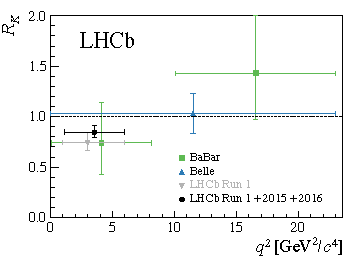
\includegraphics[width=0.7\textwidth]{\main/Flavour/figs/RKLHCb.pdf}\hbox{\hspace{-0.2cm}}\\
  \includegraphics[width=0.715\textwidth]{\main/Flavour/figs/rdrds_spring2019.png}\hbox{\hspace{-0.2cm}} 
  \caption{Upper panel: experimental results for 
  $R_K$ as function of the di-lepton invariant mass squared, $q^2$. Lower panel: status of $R_{D^{(*)}}$
  measurements; the SM predictions are  
   in tension with the experimental world average at 
  the 3.08\,$\sigma$ level \cite{HFLAVSPRING19}.}
  \label{fig:RKRD}
\end{figure}

\begin{figure}[t]
\centering
\includegraphics[width=0.45\textwidth]{\main/Flavour/figs/B2MuMu_HL-LHC.pdf}\\
\includegraphics[width=0.4\textwidth]{\main/Flavour/figs/YR_C9_C10.pdf}
\caption{ 
Upper panel: BR$(B_s^0 \to \mu^+\mu^-)$ vs. BR$(B_d^0 \to \mu^+\mu^-)$ in the SM (black cross), and in a particular supersymmetric unified model (green points are consistent with other constraints). The coloured contours show the expected $1\sigma$ \HLLHC sensitivity of ATLAS, CMS, and LHCb Upgrade~II. Lower panel: combined sensitivity of LHCb, ATLAS and CMS after the \HLLHC phase to potential new physics in $b\to s\mu\mu$ processes, motivated by recent anomalies. New physics benchmarks with leptonic vector current (new physics only in $C_9$) or pure left-handed current ($C_9=-C_{10}$), as well as the SM predictions are shown. The observables included are the branching ratio  of the $B_s\to\mu^+\mu^-$ decay and the angular observables of the decay $B^0 \to K^{\ast 0} \mu^+\mu^-$ in the low-$q^2$ region.
See  Ref.~\cite{Cerri:2018ypt} for details.}
\label{fig:Bmumu} 
\end{figure} 

In the {\bf mid-term}
the LHCb Upgrade~II, combined with the enhanced $B$-physics capabilities of ATLAS and CMS Phase~II upgrades, will enable a wide range of flavour observables to be determined at \HLLHC with unprecedented precision, complementing and extending the reach of Belle II, and of the high-p$_T$ physics programme.
Substantially improved tracking systems and the addition of timing layers in ATLAS and  CMS Phase-II detectors may significantly improve their capabilities for charged-hadron  particle identification.
The LHCb Upgrade~II will allow the experiment to run at instantaneous luminosities up to $2 \times 10^{34}{\rm cm}^{-2} {\rm s}^{-1}$ with a target integrated luminosity of 300 fb$^{-1}$, and thus exploit the full \HLLHC potential in flavour physics \cite{Bediaga:2018lhg, Cerri:2018ypt}.
Generically, and for fixed couplings, the new physics mass scale probed  will roughly double compared to the pre-\HLLHC era, see Fig.~\ref{fig:NPscales} (light vs.\ dark green for mid-term prospects with LHCb Upgrade~II).

Very recently, the suggestion that a factor of five increase in luminosity could be achieved at SuperKEKB was raised, aiming for an integrated luminosity of $250~{\rm ab}^{-1}$.
The clear complementarity of flavour physics at $e^+ e^-$ and "$pp$" colliders makes this possibility appealing. 
The major issues related to such Belle~III project  
are the feasibility from accelerator perspective and the detector challenges when running at 4 $\times 10^{36}$
cm$^{-2}$ s$^{-1}$.

The \HLLHC, combining ATLAS, CMS and LHCb Upgrade~II, has the potential to distinguish between some well-motivated  
new physics scenarios. 
The increasing precision of observables from measurements of statistically limited FCNC processes will provide significant improvements in terms of the reach to the energy scale of new-physics. 
As an example, the  plot in Fig.~\ref{fig:Bmumu} (lower panel) shows the potential sensitivity to the Wilson coefficients $C_9$ (vector current) and $C_9=-C_{10}$ (pure left-handed current), for definitions see, e.g., \cite{Aebischer:2019mlg}.
These fit results take as inputs the measurements of the branching ratio of the  $B_s\to\mu^+\mu^-$ decay and the angular observables from the decay $B^0 \to K^{\ast 0} \mu^+\mu^-$ in the low-$q^2$ region. The reach for generic new physics at tree-level is found to exceed 100~TeV, and in terms of the constraints on new-physics contributions to the $C_9$ and $C_{10}$ Wilson coefficients the study shows an approximate gain of about a factor of two compared to the constraints prior to \HLLHC. 

In addition, a wide range of lepton-universality tests in $b \to c \ell \nu$ decays can be performed, exploiting the full range of
$B$ hadrons, to probe  models of new physics.
The copious yields of semileptonic decays allow the high-precision search for CP violation in $B^0$ and $B_s$ mixing. 
In the {\bf mid-term}, the LHCb Upgrade~II dataset will allow the semileptonic asymmetries for both mesons to be measured at the level of a few $10^{-4}$, giving unprecedented new-physics sensitivity.
Precise measurements of \textbf{${\phi_s}$} and 
\textbf{${\sin 2 \beta}$} will be performed, with strategies to monitor and control possible  pollution from penguin contributions.
Advances in lattice-QCD calculations will also motivate better measurements of other critical observables, e.g., $|V_{ub}|/|V_{cb}|$, for details see Section  \ref{sec:CKM_prospects}. 

In the {\bf long-term},
at future colliders, the heavy-flavour physics is expected to be, as it is now, an integral part of the physics programme.
The new $e^+e^-$  circular colliders 
are foreseen to collect 
 $\sim 10^{ 11}$ and 
 $ \sim  10^{12}$ 
 $Z \to b \bar b$ events at 
\CEPC \cite{CEPC_INPUT} and \FCCee  \cite{Blondel:2019yqr} respectively, which  will result in all species of heavy-flavoured hadrons.
 The boosted topologies of the decay particles at the $Z$ energy, in conjunction with the clean $e^+e^-$ environment, will be beneficial for a number of measurements. 
In this respect, the $B_{s,d} \to \tau^+\tau^-$ and  $ B \to K^{(*)} \tau^+ \tau^-$ decays are  natural candidates to study. For example about 1000  events with a reconstructed  $\bar {B}^0 \to K^{*0} \tau^+\tau^-$ are expected in the $5 \times 10^{12}$ $Z$ decays at \FCCee, which would 
allow for the first investigation of  the tau lepton polarization in this mode 
\cite{Kamenik:2017ghi}. 
Recently, there has been renewed interest for the GigaZ programme at a linear collider, i.e., for runs that would collect $\sim 10^9 Z$'s from collisions with polarized electrons~\cite{Irles:2019xny}.
In general, TeraZ samples  of $\ge 10^{12} Z$'s are needed to further improve flavour-physics precision measurements and searches for rare decays after the LHCb Upgrade~II and   Belle~II (and possibly Belle~III).  
In particular, three different tests of lepton universality can be performed at a $Z$-factory. Charged current universality tests are best carried out with the $1.7 \times 10^{11}  \tau^+ \tau^-$ pairs (precision level $10^{-5}$ with TeraZ samples).
Further tests can be also performed using rare decays of heavy-flavour hadrons from the $\sim 10^{12}$ $Z\to b\bar b$  and $Z\to c \bar c$ decays.
In this case there is no benefit from the longitudinal polarization so that the polarized GigaZ sample, with three orders of magnitude fewer events, is significantly more limited. 
Neutral current universality can be tested first from the comparison of the partial widths of the $Z$ into each of the three lepton pairs; a precision better than $10^{-5}$ is expected at the TeraZ. Here again, the GigaZ will  suffer from 3000 times less statistics. 
 The ratio of vector-to-axial-vector couplings can be accessed through measurements of initial- and final-state polarization asymmetries, as well as forward-backward asymmetries. For such asymmetry measurements  the initial-state beam polarization brings substantial improvements in the reach. However, these measurements can be well performed also without longitudinal beam polarization 
 \cite{Blondel:2019yqr}.

In the \FCChh configuration, a dedicated experiment  \`{a} la LHCb could be conceived, for instance at the booster stage of the accelerator complex. Since a number of observables are expected to have negligible theoretical uncertainties even when compared with the experimental ones  after LHCb Upgrade~II, there could be a strong physics case for such an experiment.



The discussion so far focused on the physics with $b$ quarks. A related, yet different probe of new physics is offered by the {\bf charm quark decays}. In the SM, the FCNC processes involving charm hadrons are suppressed compared to those involving strange or beauty hadrons, in both the mixing and decay amplitudes. The reason is, on the one hand, that the charm quark, unlike the $b$ and $s$ quarks, can decay inside its own family. The characteristic time for the FCNC transitions is therefore much longer than the decay time, giving both $\Delta M/\Gamma\ll~1$ and $\Delta \Gamma/\Gamma\ll~1$. This fact is sustained, on the other hand, by the small breaking of the GIM mechanism controlled by the $b$ quark mass. 
The charm FCNCs can then be used as sensitive probes of new physics in the up-quark
sector, to the extent that theoretical uncertainties can be brought
under control, e.g., by constructing null tests, or circumvented by using the experimental data.

In the SM, the size of CP violation in charm decays is predicted  to be $\mathcal{O} (10^{-3} -10^{-4}$), and may be altered by  virtual new physics particles. 
The first observation of CP violation in the decay of charmed hadrons \cite{Aaij:2019kcg}
opens new opportunities across two-body, multi-body, direct and indirect CPV. The projected precisions of some analyses performed by LHCb are shown in   Fig.~\ref{fig:charm_indirect_channels} (upper panel) and are compared with the {\bf short-} and {\bf mid-term} precisions expected at Belle~II and \HLLHC. 
The available experimental measurements are also combined to establish the sensitivity to the CP-violating parameters $q/p$ and $\phi$. 
The lower plot in Fig.~\ref{fig:charm_indirect_channels}  shows the projected sensitivity with the HFLAV world average as of 2017.
At an integrated luminosity of $300\invfb$ the sensitivity to $|q/p|$ is expected to be $0.001$ and that to $\phi$ to be $0.1^\circ$.
The LHCb \upgradetwo will have the power to reach the SM estimates for $\phi$, and characterise possible new-physics contributions, if these are not too suppressed.
The charm sector investigation will be  exploited at BESIII, LHC, Belle~II (Belle~III) and \HLLHC. The programme could be complemented by some specific initiatives: TauFV at the Beam Dump at CERN \cite{TauFV_input} and $e^+e^-$ SCT factories. 
BESIII, and possibly future charm-tau factories, will exploit the $e^+e^- \to D^0 \bar {D^0}$ process to perform quantum-correlation measurements.
\begin{figure}
  \centering
  \includegraphics[width=0.85\textwidth]{\main/Flavour/figs/CharmIndirectCPVSummary.pdf}\vspace*{3mm}\\
 \includegraphics[width=0.65\textwidth]{\main/Flavour/figs/charm_indirect_CPV.pdf} 
  %
  \caption{Upper panel: Predicted constraints on the indirect CP violation
    asymmetry in
    charm from the decay channels indicated in the labels at the
    bottom of the columns. Predictions are shown in LS2
    (2020) from LHCb, LS3 (2025) from LHCb, at the end of Belle~II (2025), and at the end
    of the \HLLHC LHCb Upgrade~II\ program.
    Lower panel: Estimated constraints for LHCb \upgradetwo\ on $\phi$, $|q/p|$ from the combination of the analyses (red) compared to the current world-average precision (light blue).} 
\label{fig:charm_indirect_channels}
\end{figure}


\subsection{$\tau$ lepton: short-, mid- and long-term}
In addition to probing BSM theories, taus offer a 
good laboratory for EW precision studies and for many observables (including $|V_{us}|$, $\alpha_s(m_\tau)$ and low-energy QCD quantities)~\cite{LusianiESPP19}.

\noindent
{\bf Lepton universality tests with taus:}
these are 
powerful probes to constrain new physics models (especially those 
designed to explain LFUV anomalies).
The most precise tests rely on measurements of the tau mass,
lifetime and leptonic branching ratios, respectively 
best measured by BES III, Belle and ALEPH 
with world-average uncertainties of 0.007\%, 0.172\% and 0.178\%~\cite{Tanabashi:2018oca}.
In the {\bf short- and mid-term}, these can be improved 
by exploiting high luminosity $e^+ e^-$ colliders
like Belle II~\cite{Abe:2010gxa,Kou:2018nap} and the SCT factories. In the {\bf long-term}, 
the proposed high energy $e^+ e^-$ colliders with high
luminosity runs at the $Z$ peak (\FCCee~\cite{Blondel:2019yqr}, 
\CEPC~\cite{CEPC_INPUT}, possibly \ILC~\cite{Baer:2013cma,Fujii:2017vwa}) also offer opportunities for tests of tau lepton universality. 

{\bf Tau LFV searches:} In the {\bf short-term}, 
Belle II has a reach of
order $10^{-9}$ for $\tau \to \mu \gamma$  and 
$10^{-10}$ for $\tau \to 3 \ell$~\cite{Kou:2018nap}, corresponding to a factor 10-50 improvement. This is illustrated in Fig.~\ref{fig:NPscales} (blue), for the reach in new physics scale. 
Belle II can also search for the rare decay $\tau \to \rho \gamma$ with a projected sensitivity of $2\times 10^{-10}$ (at 50~ab$^{-1}$)~\cite{Kou:2018nap}. 
In the {\bf mid-term},  
the two SCT projects~\cite{Bondar:2013cja,Novosibirsk_SCT_input,Luo:2018njj,Peng:2018} offer favourable conditions for a competitive reach on $\tau \to \mu \gamma$. 
TauFV (planned at the Beam-Dump Facility of the
SPS, upstream of SHiP)~\cite{TauFV_input}
is a fixed-target experiment designed to search for LFV in tau decays, 
benefiting from technological developments being
pursued for the \HLLHC experiments and future hadron colliders.
TauFV's sensitivity to the $\tau \to 3 \mu$ decay
may improve that of Belle II.
In the {\bf longer term}, runs at the $Z$ pole of \FCCee (\CEPC)
can deliver 
$15\times 10^{10}$ ($3 \times 10^{10}$) $\tau$ pairs~\cite{Blondel:2019yqr, CEPC_INPUT}; 
improvements of an
order of magnitude with respect to Belle II may thus be possible. 


{\bf Precision tau measurements:}
In the {\bf short-term}, Belle II has the potential for improvements,
at the price of considerable work on the limiting systematics. 
In the {\bf mid-term}, the programmes of the STC factories include precision
measurements of low multiplicity tau branching ratios, and
offer by far the best prospects regarding tau mass measurements~\cite{Bondar:2013cja,Novosibirsk_SCT_input,Luo:2018njj,Peng:2018}: 
$\Delta m_\tau = \pm 0.012$~MeV, due to a reduction of systematic errors
(for Belle II, 
$\Delta m_\tau = 
\pm 0.10 - 0.15$~MeV~\cite{Kou:2018nap}). 
In the {\bf long term}, future $e^+ e^-$ colliders operating at the $Z^0$
pole offer the best conditions for significant advances. 
For BR($\tau \to \ell \bar \nu\nu$), 
 both \FCCee and \CEPC can
reach a precision of 0.02\%~\cite{Blondel:2019yqr,CEPC_INPUT}. For the tau lifetime, 
\FCCee aims at a precision  
$\Delta \tau_\tau \sim 0.01\%$ 
(to be compared with 0.026\% at Belle II). For tau mass measurements, \FCCee is less performant than the other possible projects: 
by calibrating on $m_{D^+}$, it aims at 
$\Delta m_\tau = 0.07$~MeV.


A  summary of the above sensitivity goals and prospects concerning $\tau \to 3\mu$ decays and $m_\tau$ can be found in Fig.~\ref{fig:Lusiani_prospects}.

\begin{figure}
\centering
\hspace*{-3mm}
\includegraphics[width=0.75\textwidth]{\main/Flavour/figs/ul90cl-tau-3mu-esg-may19} 
\vspace*{3mm}\\
\includegraphics[width=0.75\textwidth]{\main/Flavour/figs/unc-tau-mass-esg-may19} 
\caption{Expected sensitivity and projected precision of  present and future experiments for $\tau \to 3\mu$ decays and $m_\tau$~\cite{LusianiESPP19}.
Green denotes current measurements, red  points correspond to estimates of future experimental sensitivities based on dedicated studies (relying on extrapolation from past established performances) while orange corresponds to estimates of experimental sensitivities including novel features (for which extrapolation from past experience is more difficult). }\label{fig:Lusiani_prospects} 
\end{figure}

\subsection{The Higgs, top quark, gauge bosons (short-, mid- and long-term)}
 In the SM the flavour structure is encoded in 
 the Higgs couplings to the fermions. 
 
\textbf{ Fermion masses.} In the SM the  
diagonalized Yukawa couplings, $y_f$, are
proportional to the fermion masses, $m_f$,  with a common
factor,  $y_f = \sqrt{2} \kappa_f m_f / v$, where  $\kappa_f^{\rm SM}=1$;
moreover,
there are no tree-level flavour changing couplings of the Higgs. This may change in the presence of new physics, in which case the couplings of the Higgs to the fermions can in general take the form, $\mathcal{L}_{\rm eff} = -\kappa_{f_i} (m_{f_i}/{v}) h \bar f_i f_i + i \tilde \kappa_{f_i} (m_{f_i}/v) h \bar f_i \gamma_5 f_i  
	- \big[\big( \kappa_{f_i f_j} + i \tilde \kappa_{f_i f_j} \big) h \bar f_L^i f_R^j +{\rm h.c.}\big]_{i\neq j}. $
	Currently, only the third generation Yukawa couplings have been measured, having been found to be in agreement with the SM predictions, while for the Higgs couplings to the first two generations, only upper bounds exist. 
Experimentally, a number of SM predictions for the Higgs couplings to fermions 
must be tested as precisely as possible: {\em (i)} proportionality, $y_f\propto m_f$; {\em (ii)} the factor of proportionality, $\kappa_{f_i}=1$; {\em (iii)} diagonality (no off-diagonal flavour violating couplings at tree level, $\kappa_{f_i f_j}=\tilde \kappa_{f_i f_j}= 0$); {\em (iv)} reality (no CP violation at tree level, $\tilde \kappa_{f_i}=\tilde \kappa_{f_i f_j}=0$) \cite{Nir:2016zkd}.

\begin{figure}[t]
	\centering
	\includegraphics[width=0.75\textwidth]{\main/Flavour/figs/kappaplot}\vspace*{3mm}\\
       \includegraphics[width=0.75\textwidth]{\main/Flavour/figs/BrplotFV}
	\caption{Summary of the  projections for measurements of Higgs Yukawa couplings to quarks and leptons (upper panel), and on select flavour violating decays (lower panel), adapted from Ref.~\cite{Heinemann:2019trx}. 
	\label{fig:higgs:forecast}}
\end{figure}
The summary of the expected experimental sensitivies is shown in Fig.~\ref{fig:higgs:forecast} (upper panel) using the $\kappa_f$ framework as a toy approximation to show sensitivity in each channel (a global view of experimental constraints using SM-EFT can be found in \cite{deBlas:2019rxi}). 
The sensitivity in the muon channel is now close to what is required to test the SM prediction for the muon Yukawa. This will be the first meaningful test of the 2nd generation Yukawa couplings. A precision measurement does require larger datasets that will be provided in the {\bf short- and mid-term} by the LHC in Run 3 and by the \HLLHC.
In the {\bf mid-term}, the \HLLHC will bound the Yukawa couplings to the third generation fermions and to the muon to a few percent level. 
In the {\bf long-term}, the proposed large scale experiments, \ILC, \FCCee, \CEPC, and \CLIC can significantly improve this precision, to below percent level. They would also measure the charm Yukawa coupling for the first time, and probe it quite precisely, at the percent level. A slightly more modest improvement can be expected at the \HELHC \cite{deBlas:2019rxi}. 
In addition, at \FCCee the upper bound of $\delta y_e/y_e<1.6$ can be achieved after
one year of running at $\sqrt{s}=m_h$. 

\textbf{ Flavour violating Higgs decays}: for the branching ratios of $h\to \tau\mu, \tau e$ decays,  in the {\bf mid-term}  \HLLHC is expected to improve the reach by an order of magnitude, to the level of $5\times 10^{-4}$, see Fig.~\ref{fig:higgs:forecast} (lower panel).  
Figure~\ref{fig:NPscales} illustrates in light (dark) red the scale reach of present data (\HLLHC prospects). Taking $h\to \mu\mu$ and $h\to \tau\tau$ as guidance, one can expect {\bf in the long term} another one to two orders of magnitude improvements for $h\to \tau\mu$ at \FCChh \cite{deBlas:2019rxi}.


\textbf{The top quark} is unique among the SM fermions, with its ${\mathcal O}(1)$ coupling to the Higgs. Such a large Yukawa coupling for the top is also the origin of the weak scale hierarchy problem -- the quadratically divergent corrections to the Higgs mass are a problem precisely because of it. 
It is thus very common for new physics models that address the  hierarchy problem to also lead to modifications of the top quark properties.  
Studying precisely the latter may in addition give insight into the origin of the SM flavour puzzle, or at least as to why one and only one Yukawa coupling is large.  Experimentally, new physics is probed using FCNC top decays, $t\to c\gamma, cZ, cg, ch$. 
The present upper bounds on their branching ratios are in the range $10^{-3}-10^{-4}$, and will be improved by an order of magnitude or more in the {\bf mid-term} at \HLLHC, resulting in about a two-fold increase in the reach to the effective new physics scale, cf. Fig. \ref{fig:NPscales}.
Also in the mid-term, the reach for  $t\to hc, hu$ decays is expected to improve  by one order of magnitude from the present $10^{-3}$ level,   at \HLLHC; see Fig.~\ref{fig:NPscales} (dark red) for the corresponding sensitivity to new physics scales. This is expected to be further improved in the {\bf long-term}  at \FCChh, see Fig.~\ref{fig:higgs:forecast} (lower panel).

\textbf{The $Z$ boson} is also a sensitive probe of new physics: for instance, the observation of flavour violating $Z\to e\mu, \mu\tau, e\tau$ decays would be a clear evidence of new physics, for instance, the existence of sterile neutral fermions. The current limits on these decays are ${\mathcal O}(10^{-6}-10^{-5})$, and could be improved by several orders of magnitude, down to ${\mathcal O}(10^{-9})$ at \FCCee \cite{Abada:2019lih}. 


Lepton flavour violating transitions such as $e^+e^-\to e^+\tau^-$ would also probe \textbf{contact interactions}. The LFV operators of the schematic form $(\bar e e)(\bar e \tau)$ could be well probed at future high energy $e^+e^-$ colliders, and would increase the present bound of $\sim9$~TeV (on the scale of the contact interaction) to 35~TeV at a \CLIC running at 3~TeV~\cite{deBlas:2018mhx}. 




\section{Flavour and dark sectors (short-, mid- and long-term)}



Flavour physics could be instrumental in searches for dark matter or dark sectors. Light dark sector particles can be produced in \textbf{flavour violating rare decays}, for instance in $B\to K X_{\rm dark}$, $B\to D X_{\rm dark}$, $D\to K X_{\rm dark}$, $K\to \pi X_{\rm dark}$, either through tree level or one loop mediated emissions of dark sector particles, see, e.g., Refs.~\cite{Bird:2004ts,Kamenik:2011vy}. Such decays are an exciting and increasingly important drivers in the searches for dark sector candidates, since they are often the dominant production channels. Particles that 
either carry nonzero flavour or have flavour violating couplings  may  thus be produced in the flavour violating transitions at tree level, as for instance, heavy neutral leptons \cite{Gorbunov:2007ak} and the  axiflavon~\cite{Calibbi:2016hwq,Ema:2016ops,Wilczek:1982rv}. 
Examples of particles with flavour diagonal couplings, produced in meson decays induced at one loop via $W^\pm$ exchange, include a light singlet scalar mixing with the Higgs~\cite{OConnell:2006rsp,Batell:2009jf,Winkler:2018qyg},  ALPs (axion-like particles)~\cite{Jaeckel:2010ni}, and some dark matter candidates. It is  interesting that even the experiments whose primary goals are in flavour physics, such as NA62 or the Upgrade II of LHCb, have significant discovery potential in dark sector searches. 

The dark sector particles in the final state, $X_{\rm dark}$, may decay back into visible particles and be detected or, alternatively, result in missing energy and momentum, if they are sufficiently long-lived
or decay to neutrinos. 
When visible, the vertex may be prompt or displaced, depending on the lifetime of $X_{\rm dark}$.   There are a number of proposed experiments, with a clear synergy between different search strategies, such as searches for displaced vertices, monojets, etc. In the {\bf short-term}  the existing and approved experiments, Faser~\cite{Feng:2017uoz}, NA62~\cite{Gonnella:2017hsz}, NA64~\cite{Banerjee:2016tad}, SeaQuest~\cite{Berlin:2018pwi}, LHCb, ATLAS and CMS could explore different dark sector models. In the {\bf mid-term} the proposed experiments, such as beam dump mode of NA62~\cite{Beacham:2019nyx}, LHCb combined with Codex-b~\cite{Gligorov:2017nwh}, Belle II combined with Gazelle, LDMX~\cite{Akesson:2018vlm}, Mathusla~\cite{Chou:2016lxi,Alpigiani:2018fgd}, and SHiP~\cite{Alekhin:2015byh}   could explore large regions of presently unconstrained parameter space, see Fig.~\ref{fig:dark:daulepton} for two examples. 
  Also in the mid-term, Upgrade II of LHCb will have improved sensitivity to dark photons from $D^*\to D\gamma_{\rm dark}$ decays or from bump hunting in the $\mu^+\mu^-$ spectra. In the {\bf long-term}  \FCCee  could significantly increase the reach for dark sector masses, e.g. to a further order of magnitude in mass. 

The  sensitivity of the proposed experiments  to {\bf heavy neutral leptons} mixing with active neutrino flavours is discussed in Sect.~\ref{hnl-sec-nu}.  The  reach for the case in which they mix predominantly with the electron or with the tau flavour, as well as the present bounds (shaded regions), are  illustrated in Fig.~\ref{fig:FIPs-HNL} and  Fig.~\ref{fig:dark:daulepton} (upper panel), respectively.  There is clearly a very strong potential for a whole suite of experiments. 
%Similarly is true of 
The same holds for other sample models, for instance for a {\bf Higgs-mixed singlet scalar} $S$, shown in Fig.~\ref{fig:dark:daulepton} (lower panel). While smaller scale experiments such as NA62++, FASER and CODEX-b can cover substantial parts of the parameter space for light new dark sectors, the two
 experiments proposed in this regime
  with larger (and comparable) reach in many models  
 are MATHUSLA and SHiP. MATHUSLA and CODEX-b can also probe dark sector particles with masses above few GeV if they originate from decays of heavier states, such as $h\to SS$ decays as illustrated in  Fig.~\ref{fig:dark:daulepton} (lower panel). Overall, the combination of LHCb Upgrade II and CODEX-b, and of ATLAS/CMS and MATHUSLA would cover a very diverse and wide range of new physics options. Heavier dark sectors can be probed in the long-term at \FCCee and/or \CEPC relying on their expected large numbers of $Z$ decays. 


\begin{figure}[t]
	\centering 
	\includegraphics[width=0.8\textwidth]{\main/Flavour/figs/HNL_bc8_pbc_2.png}\\
	\includegraphics[width=0.8\textwidth]{\main/Flavour/figs/BC5_pbc_2.png}
	\caption{Reach of proposed experiments for heavy neutral leptons coupling predominantly to the tau flavour (top panel) and for Higgs-mixed scalar (bottom panel). From Ref.\cite{Beacham:2019nyx}.	
	\label{fig:dark:daulepton}}
\end{figure}

There is also sensitivity to dark sector mediators in \textbf{classical flavour observables} such as \textbf{meson mixings},  or \textbf{${(g-2)}$ of the muon}. They can contribute at tree-level, in which case the flavour experiments can probe very high scales for ${\mathcal O}(1)$ couplings, or at loop-level as is the case for some   DM candidates and the accompanying $Z_2$-odd mediators. 

An intriguing possibility is that flavour physics might be directly involved in the structure of the dark sector or in its cosmological consequences. For instance, the stability of dark matter could be due to flavour symmetries; striking examples of cosmological consequences of flavour structures are the option of low-scale ($1-100$ GeV) baryogenesis via heavy neutral leptons~\cite{Akhmedov:1998qx,Asaka:2005pn}, or 
having CP violation solely from the SM sector through meson mixing oscillations, whose signature would be seemingly baryon-violating flavour transitions with missing energy (such as $B\to \Lambda 
X_{\rm dark}$)~\cite{Nelson:2019fln,Elor:2018twp}. 
 Conversely, a better understanding of 
 the SM flavour puzzle could potentially come by studying the flavour structure of dark sector.




\section{The CKM matrix elements: prospects}\label{sec:CKM}
\label{sec:CKM_prospects}

Weak charged currents mix quarks of different generations. In the SM, the strengths of the corresponding transitions are encoded in the unitary Cabibbo-Kobayashi-Maskawa (CKM) matrix~\cite{Cabibbo:1963yz,Kobayashi:1973fv}.
Unitarity, in conjunction with invariance under field redefinitions, implies that all nine complex elements of the  $3\times 3$ CKM matrix are described by four physical parameters. 
In turn, this implies relations between different CKM elements, such as the closure of the standard CKM unitarity triangle (which may not hold  in the presence of new physics).  
Overconstraining the apex of the unitarity triangle from tree- and loop-level quark mixing processes is therefore a powerful way to probe for virtual new physics effects that may arise from mass scales above those which can be directly searched for at colliders. In many cases such indirect probes of new physics will not be limited by either experimental or theoretical systematics at least in the {\bf mid-term}, i.e., in the \HLLHC era, and potentially even for any {\bf long-term} programs (see Table \ref{table:Proj} for expected improvements in lattice QCD for a selection of observables).


\begin{table}
\caption{Current estimates and projections for experimental reach for a selection of observables at Belle~II and LHCb, including Upgrade~II, compared to lattice QCD determinations of hadronic inputs for the {\bf short-} and {\bf mid-term}, taken to be, respectively, the Phase I and II stages defined in Ref.~\cite{Cerri:2018ypt}. It is assumed that the QED corrections to lattice QCD results will be calculated. For a more complete listing of lattice QCD projections see Table 42 of Ref.~\cite{Cerri:2018ypt}.}
    \label{table:Proj}
    {\footnotesize
\begin{center}
\begin{tabular}{ccccc}
\hline\hline
Quantity & Ref. &present error & short-term & mid-term\\
\hline
$(\Delta m_s/\Delta m_d)_{\rm exp}$ & \cite{Tanabashi:2018oca} & $0.4\%$ & - & -
\\
$\xi$ for $(\Delta m_s/\Delta m_d)_{\rm theor}$ & \cite{Cerri:2018ypt} & $1.4\%$ & $0.3\%$ & $0.3\%$
\\
\hline
$B\to \pi$: $|V_{ub}|_{{\rm exp}}$ & \cite{Cerri:2018ypt,Bediaga:2018lhg,Kou:2018nap} &    $2.3\%$ & $1.6\%$ & $1.1\%$\\
$B\to \pi$: $|V_{ub}|_{{\rm theor}}$ & \cite{Cerri:2018ypt} &    $2.9\%$ & $1\%$ & $1\%$\\
\hline
$B\to D$: $|V_{cb}|_{{\rm exp}}$& \cite{Cerri:2018ypt,Kou:2018nap} &   $ 2.0\%$ & $1.4\%$ & -\\
$B\to D$: $|V_{cb}|_{{\rm theor}}$&\cite{Cerri:2018ypt} &    $1.4\%$ & $0.3\%$ & $0.3\%$\\
\hline
$B\to D^*$: $|V_{cb}|_{{\rm exp}}$ & \cite{Kou:2018nap}& $1.2\%$ &- & - \\ 
$B\to D^*$: $|V_{cb}|_{{\rm theor}}$ & \cite{Cerri:2018ypt}& $1.4\%$ & $0.4\%$ & $0.4\%$ \\  
\hline
$\Lambda_b\to p(\Lambda_c)$: $|V_{ub}/V_{cb}|_{{\rm exp}}$ & \cite{Bediaga:2018lhg} &   $ 6\%$ & $1\%$ & $1\%$\\
$\Lambda_b\to p(\Lambda_c)$: $|V_{ub}/V_{cb}|_{{\rm theor}}$  &\cite{Cerri:2018ypt} & $4.9\%$ & $1.2\%$ & $1.2\%$\\
\hline
\hline
\end{tabular}
\end{center}
}
\end{table}

\begin{table}
\caption{Relative uncertainties on the predictions of UT parameters and angles, using current and extrapolated input values for measurements and theoretical parameters (UTfit collaboration, from~\cite{Cerri:2018ypt}, with short-(mid-)term taken as Phase I(II) stages defined in~\cite{Cerri:2018ypt}).}
\label{tab:utfit_global}
{\footnotesize
 \begin{center}
       \begin{tabular}{ccccccccc}
               \hline\hline
                & $\lambda$ & $\bar{\rho}$ & $\bar{\eta}$ & $A$ & $\sin2\beta$ & $\gamma$ & $\alpha$ & $\beta_s$ \\ \hline
                       Current &0.12\%& 9\% & 3\% & 1.5\% & 4.5\% & 3\% & 2.5\% & 3\% \\
                       short-term  &0.12\%& 2\% & 0.8\% & 0.6\% & 0.9\% &  0.9\% & 0.7\% & 0.8\%\\
                       mid-term  &0.12\%& 1\% & 0.6\% & 0.5\% & 0.6\% & 0.8\% & 0.4\% & 0.5\%\\ \hline
       \hline
       \end{tabular}
\end{center}
}
\end{table}



Figure~\ref{fig:UTprojection} shows the projected {\bf short-} and {\bf mid-term} improvements on constraints in the plane of two unitarity triangle parameters, $\bar{\rho}$ and $\bar{\eta}$, using only expected improvements in LHCb inputs and lattice-QCD calculations, while Table \ref{tab:utfit_global} gives the expected improvements by using both LHCb and Belle-II results. The increased sensitivity will allow for extremely precise tests of the CKM paradigm. In particular, it will permit the tree-level observables, which provide the SM benchmarks, to  be assessed against  those with loop contributions, which are more susceptible to new physics.  In practice, this already very powerful ensemble of constraints will be 
further strengthened by complementary measurements from Belle II, particularly in the case of $|V_{ub}|$ and $|V_{cb}|$, where $\sim $1\% precision is expected. Improvement on the determination of $|V_{cb}|$ will also greatly impact the constraints on the CKM matrix elements that follow from the measurement of $\varepsilon_K$.

\begin{figure}[t]
\begin{center}
\includegraphics[width=0.65\textwidth]{Flavour/figs/rhoeta_small_LHCb_Summer18.pdf}

\begin{minipage}{0.65\textwidth}
\includegraphics[width=\textwidth]{Flavour/figs/rhoeta_small_LHCb_Stage1.pdf}\vspace{-5.36cm}
\mbox{\hspace{7.9cm}\includegraphics[width=0.26\textwidth]{Flavour/figs/rhoeta_small_zoom_LHCb_Stage1.pdf}}
\vspace{2.25cm}
\end{minipage}

\begin{minipage}{0.65\textwidth}
\includegraphics[width=\textwidth]{Flavour/figs/rhoeta_small_LHCb_Stage2.pdf}\vspace{-5.36cm}
\mbox{\hspace{7.9cm}\includegraphics[width=0.26\textwidth]{Flavour/figs/rhoeta_small_zoom_LHCb_Stage2.pdf}}
\vspace{2.25cm}
\end{minipage}

\caption{\small  Evolving constraints in the $\bar{\rho}-\bar{\eta}$ plane from LHCb measurements and lattice QCD calculations, alone, with current inputs (2018), and the anticipated improvements from the data accumulated by 2025  (23\,fb$^{-1}$) and 2035 (300\,fb$^{-1}$), from top to bottom, respectively.
Figures from Ref.~\cite{Bediaga:2018lhg}. }
\label{fig:UTprojection}
\end{center}
\end{figure} 

The \textbf{angle} $\pmb{\gamma}$ is currently the least well known CKM parameter ($\pm 5^\circ$).
In the {\bf short-term} both LHCb Upgrade~I and Belle ~II will provide measurements at $\sim$ 1.5 $^\circ$. In the {\bf mid-term} LHCb Upgrade~II will allow for a  sensitivity at the sub-degree level.
The best sensitivity to $\gamma$ is from $B\to DK$ decays. The anticipated largest systematic uncertainty will be due to the external inputs on the strong phase differences in $D$ meson decays, for which 
BES~III and the SCT factories are expected to provide precise measurements.  Table~\ref{tab:utfit_global} shows the foreseen {\bf mid-term} impact of experimental and theoretical developments on global CKM fits, as estimated by the UTFit group~\cite{Cerri:2018ypt} (comparable CKMfitter estimates can also be found in Ref.~\cite{Cerri:2018ypt}).

The precision measurement of the $B_s$ weak mixing phase, $\phi_s$, will be another highlight of the {\bf mid-term} programme. The expected precision on $\phi_s^{c\bar{c}s}$ at the end of \HLLHC  will be $\sim 5$~mrad for ATLAS and CMS, and $\sim 3$~mrad for LHCb. 
This determination of $\phi_s$ from a loop induced process susceptible to new physics, will be at the same level of precision as the current one on the indirect determination (based on the CKM fit using tree-level measurements). This allows for a precise probe of new physics contributions.






\section{Conclusions}

 Since the last update of the European Strategy, a plethora of new experimental results  has been achieved in flavour physics.  No indisputable evidence of new physics has  emerged so far,  though. 
 The rationale for the observed pattern of masses and mixings of quarks and leptons thus still remains a fundamental open question, which calls for new physics laws.  Precision flavour physics is a fundamental tool to discover them.


  The probing power of flavour physics is manifest from the comparative effective analysis of Fig.~\ref{fig:NPscales}. In the near future, the sensitivities of several observables will reach very high NP scales, $10^2-10^5$~TeV -- scales which are beyond the reach of high-energy colliders.  Note that this analysis does not claim that physics at --or below-- the  scale depicted is guaranteed to provide a measurable deviation from the SM.  All we claim is that a new physics scale  might be first signalled via 
flavour measurements. In spite of its 
 caveats, the figure illustrates well the great physics reach of flavour observables versus that of  direct and electroweak precision searches. Overall, these three quests are complementary and essential.  

 

The field of flavour has been traditionally explored through a wide spectrum of experiments, ranging from low- and intermediate-energies, such as  EDMs, dedicated muon, kaon, tau, charm and beauty experiments, to the high-energy frontier (the LHC experiments), all the way to feebly interacting particle searches. Measurements by these diverse experiments and facilities lead to valuable complementary information on the different pieces required to assemble the flavour physics mosaic. 

In the \textbf{short- and mid-term}, the expected progress of running experiments, the sensitivity goals of those already foreseen and the proposed upgrades of existing ones, will enable to determine a wide range of flavour observables with unprecedented precision (or establish new impressive limits).

Searches for EDMs of various types of particles are currently being performed. 
Substantial improvements in the short and mid-term are expected: the neutron and proton EDMs down to $10^{-29} $ e$\cdot$cm, and  $10^{-30} $ e$\cdot$cm  for the electron. Dedicated searches for charged lepton flavour violation in the muon sector foresee nominal improvements by as much as a factor of $10\,000$,  owing to the  high-intensity muon beam programmes at PSI, FNAL and J-PARC.   Furthermore, current hints of lepton non-universality in both charged-current and neutral-current semileptonic $B$ decays are expected to be  unambiguously tested.


In the quark flavour arena, kaon physics proceeds with a steady pace of improvements: efforts towards a substantial improvement on sensitivity for the $K^+ \to \pi^+ \nu \bar \nu$ decay 
and a first measurement of the $K_L \to \pi^0 \nu \bar \nu$ decay are underway.  The upcoming results expected from NA62 and the evolution of the Japanese project will guide the future European steps in this research field. 
Heavy quarks, and in general heavy flavour physics will continue to play an important role also in the post-LHC era. Furthermore, the improvements in lattice-QCD calculations are expected to keep pace with advances in  experimental precision,  
 motivating better measurements of observables critical to test the CKM paradigm.  A flourishing new area is also opening in the mid-term for the exploration of NP in flavourful Higgs couplings, as well as in top and gauge boson interactions. 

The LHCb Upgrade II would allow 
 for the full exploitation of the flavour physics potential of \HLLHC  and increase the explored NP mass scale by close to a factor two with respect to the short-term LHCb Upgrade~I.
It would also provide a bridge towards larger scale collider facilities.
Analogous considerations are valid for a possible upgrade of Belle II (Belle III).
Essential to the success of the physics programme is the experiment capability of charge particle identification and systematic uncertainty control
in different  environments 
($pp$  and $e^+e^-$).


In the \textbf{long-term}, experiments at a future high-luminosity $e^+e^-$ collider 
would perform unique heavy-flavour studies 
in specific channels. 
Circular colliders operating at the $Z$  
pole (in particular \FCCee) 
can strongly contribute to develop searches for  the charm Yukawa coupling and flavour-violating Higgs and $Z$ couplings, lepton flavour violation and precision tau physics, and dark sector searches.   
At a circular high-energy $pp$ collider, the top Yukawa coupling, flavour-violating top-Higgs couplings,  and other heavy flavour physics program related to $b$ and $c$ quark decays would be best studied with a dedicated experiment, along the lines of LHCb.



Furthermore,  from both the experimental and the theory side, a novel synergy  between the searches for flavour violating decays and that  for feebly interacting and dark particles is emerging. Searching for exotic signatures in flavour violating decays  
may have profound implications for our understanding of the Universe, and should be part of any broad program of searches for dark sectors. 
 High energy colliders will explore a large number of signatures and cover a large fraction of the parameter space for the high-mass range (above 10~GeV). 
Nevertheless fixed target smaller scale experiments, LHC projects dedicated
to long-lived particles and beam dump facilities may provide complementary information to explore a lower mass range  
(1~MeV - 10~GeV) and open new interesting research lines. 

\bigskip
The foreseen unprecedented improvements in sensitivity, together with the novel  channels to be explored, will make  the next decade particularly exciting for the flavour physics arena. 
In summary, the combination of
quark and lepton searches 
for flavour and CP violation  
 at different frontiers is 
a formidable tool to discover new physics. 
Flavour physics must be a crucial ingredient of the future strategy of particle physics. 




\end{document}

